\documentclass{article}
\usepackage{iclr2027_conference,times}
\renewcommand{\ttdefault}{cmtt}
%%%%% NEW MATH DEFINITIONS %%%%%

\usepackage{amsmath,amsfonts,bm}

% Mark sections of captions for referring to divisions of figures
\newcommand{\figleft}{{\em (Left)}}
\newcommand{\figcenter}{{\em (Center)}}
\newcommand{\figright}{{\em (Right)}}
\newcommand{\figtop}{{\em (Top)}}
\newcommand{\figbottom}{{\em (Bottom)}}
\newcommand{\captiona}{{\em (a)}}
\newcommand{\captionb}{{\em (b)}}
\newcommand{\captionc}{{\em (c)}}
\newcommand{\captiond}{{\em (d)}}

% Highlight a newly defined term
\newcommand{\newterm}[1]{{\bf #1}}


% Figure reference, lower-case.
\def\figref#1{figure~\ref{#1}}
% Figure reference, capital. For start of sentence
\def\Figref#1{Figure~\ref{#1}}
\def\twofigref#1#2{figures \ref{#1} and \ref{#2}}
\def\quadfigref#1#2#3#4{figures \ref{#1}, \ref{#2}, \ref{#3} and \ref{#4}}
% Section reference, lower-case.
\def\secref#1{section~\ref{#1}}
% Section reference, capital.
\def\Secref#1{Section~\ref{#1}}
% Reference to two sections.
\def\twosecrefs#1#2{sections \ref{#1} and \ref{#2}}
% Reference to three sections.
\def\secrefs#1#2#3{sections \ref{#1}, \ref{#2} and \ref{#3}}
% Reference to an equation, lower-case.
\def\eqref#1{equation~\ref{#1}}
% Reference to an equation, upper case
\def\Eqref#1{Equation~\ref{#1}}
% A raw reference to an equation---avoid using if possible
\def\plaineqref#1{\ref{#1}}
% Reference to a chapter, lower-case.
\def\chapref#1{chapter~\ref{#1}}
% Reference to an equation, upper case.
\def\Chapref#1{Chapter~\ref{#1}}
% Reference to a range of chapters
\def\rangechapref#1#2{chapters\ref{#1}--\ref{#2}}
% Reference to an algorithm, lower-case.
\def\algref#1{algorithm~\ref{#1}}
% Reference to an algorithm, upper case.
\def\Algref#1{Algorithm~\ref{#1}}
\def\twoalgref#1#2{algorithms \ref{#1} and \ref{#2}}
\def\Twoalgref#1#2{Algorithms \ref{#1} and \ref{#2}}
% Reference to a part, lower case
\def\partref#1{part~\ref{#1}}
% Reference to a part, upper case
\def\Partref#1{Part~\ref{#1}}
\def\twopartref#1#2{parts \ref{#1} and \ref{#2}}

\def\ceil#1{\lceil #1 \rceil}
\def\floor#1{\lfloor #1 \rfloor}
\def\1{\bm{1}}
\newcommand{\train}{\mathcal{D}}
\newcommand{\valid}{\mathcal{D_{\mathrm{valid}}}}
\newcommand{\test}{\mathcal{D_{\mathrm{test}}}}

\def\eps{{\epsilon}}


% Random variables
\def\reta{{\textnormal{$\eta$}}}
\def\ra{{\textnormal{a}}}
\def\rb{{\textnormal{b}}}
\def\rc{{\textnormal{c}}}
\def\rd{{\textnormal{d}}}
\def\re{{\textnormal{e}}}
\def\rf{{\textnormal{f}}}
\def\rg{{\textnormal{g}}}
\def\rh{{\textnormal{h}}}
\def\ri{{\textnormal{i}}}
\def\rj{{\textnormal{j}}}
\def\rk{{\textnormal{k}}}
\def\rl{{\textnormal{l}}}
% rm is already a command, just don't name any random variables m
\def\rn{{\textnormal{n}}}
\def\ro{{\textnormal{o}}}
\def\rp{{\textnormal{p}}}
\def\rq{{\textnormal{q}}}
\def\rr{{\textnormal{r}}}
\def\rs{{\textnormal{s}}}
\def\rt{{\textnormal{t}}}
\def\ru{{\textnormal{u}}}
\def\rv{{\textnormal{v}}}
\def\rw{{\textnormal{w}}}
\def\rx{{\textnormal{x}}}
\def\ry{{\textnormal{y}}}
\def\rz{{\textnormal{z}}}

% Random vectors
\def\rvepsilon{{\mathbf{\epsilon}}}
\def\rvtheta{{\mathbf{\theta}}}
\def\rva{{\mathbf{a}}}
\def\rvb{{\mathbf{b}}}
\def\rvc{{\mathbf{c}}}
\def\rvd{{\mathbf{d}}}
\def\rve{{\mathbf{e}}}
\def\rvf{{\mathbf{f}}}
\def\rvg{{\mathbf{g}}}
\def\rvh{{\mathbf{h}}}
\def\rvu{{\mathbf{i}}}
\def\rvj{{\mathbf{j}}}
\def\rvk{{\mathbf{k}}}
\def\rvl{{\mathbf{l}}}
\def\rvm{{\mathbf{m}}}
\def\rvn{{\mathbf{n}}}
\def\rvo{{\mathbf{o}}}
\def\rvp{{\mathbf{p}}}
\def\rvq{{\mathbf{q}}}
\def\rvr{{\mathbf{r}}}
\def\rvs{{\mathbf{s}}}
\def\rvt{{\mathbf{t}}}
\def\rvu{{\mathbf{u}}}
\def\rvv{{\mathbf{v}}}
\def\rvw{{\mathbf{w}}}
\def\rvx{{\mathbf{x}}}
\def\rvy{{\mathbf{y}}}
\def\rvz{{\mathbf{z}}}

% Elements of random vectors
\def\erva{{\textnormal{a}}}
\def\ervb{{\textnormal{b}}}
\def\ervc{{\textnormal{c}}}
\def\ervd{{\textnormal{d}}}
\def\erve{{\textnormal{e}}}
\def\ervf{{\textnormal{f}}}
\def\ervg{{\textnormal{g}}}
\def\ervh{{\textnormal{h}}}
\def\ervi{{\textnormal{i}}}
\def\ervj{{\textnormal{j}}}
\def\ervk{{\textnormal{k}}}
\def\ervl{{\textnormal{l}}}
\def\ervm{{\textnormal{m}}}
\def\ervn{{\textnormal{n}}}
\def\ervo{{\textnormal{o}}}
\def\ervp{{\textnormal{p}}}
\def\ervq{{\textnormal{q}}}
\def\ervr{{\textnormal{r}}}
\def\ervs{{\textnormal{s}}}
\def\ervt{{\textnormal{t}}}
\def\ervu{{\textnormal{u}}}
\def\ervv{{\textnormal{v}}}
\def\ervw{{\textnormal{w}}}
\def\ervx{{\textnormal{x}}}
\def\ervy{{\textnormal{y}}}
\def\ervz{{\textnormal{z}}}

% Random matrices
\def\rmA{{\mathbf{A}}}
\def\rmB{{\mathbf{B}}}
\def\rmC{{\mathbf{C}}}
\def\rmD{{\mathbf{D}}}
\def\rmE{{\mathbf{E}}}
\def\rmF{{\mathbf{F}}}
\def\rmG{{\mathbf{G}}}
\def\rmH{{\mathbf{H}}}
\def\rmI{{\mathbf{I}}}
\def\rmJ{{\mathbf{J}}}
\def\rmK{{\mathbf{K}}}
\def\rmL{{\mathbf{L}}}
\def\rmM{{\mathbf{M}}}
\def\rmN{{\mathbf{N}}}
\def\rmO{{\mathbf{O}}}
\def\rmP{{\mathbf{P}}}
\def\rmQ{{\mathbf{Q}}}
\def\rmR{{\mathbf{R}}}
\def\rmS{{\mathbf{S}}}
\def\rmT{{\mathbf{T}}}
\def\rmU{{\mathbf{U}}}
\def\rmV{{\mathbf{V}}}
\def\rmW{{\mathbf{W}}}
\def\rmX{{\mathbf{X}}}
\def\rmY{{\mathbf{Y}}}
\def\rmZ{{\mathbf{Z}}}

% Elements of random matrices
\def\ermA{{\textnormal{A}}}
\def\ermB{{\textnormal{B}}}
\def\ermC{{\textnormal{C}}}
\def\ermD{{\textnormal{D}}}
\def\ermE{{\textnormal{E}}}
\def\ermF{{\textnormal{F}}}
\def\ermG{{\textnormal{G}}}
\def\ermH{{\textnormal{H}}}
\def\ermI{{\textnormal{I}}}
\def\ermJ{{\textnormal{J}}}
\def\ermK{{\textnormal{K}}}
\def\ermL{{\textnormal{L}}}
\def\ermM{{\textnormal{M}}}
\def\ermN{{\textnormal{N}}}
\def\ermO{{\textnormal{O}}}
\def\ermP{{\textnormal{P}}}
\def\ermQ{{\textnormal{Q}}}
\def\ermR{{\textnormal{R}}}
\def\ermS{{\textnormal{S}}}
\def\ermT{{\textnormal{T}}}
\def\ermU{{\textnormal{U}}}
\def\ermV{{\textnormal{V}}}
\def\ermW{{\textnormal{W}}}
\def\ermX{{\textnormal{X}}}
\def\ermY{{\textnormal{Y}}}
\def\ermZ{{\textnormal{Z}}}

% Vectors
\def\vzero{{\bm{0}}}
\def\vone{{\bm{1}}}
\def\vmu{{\bm{\mu}}}
\def\vtheta{{\bm{\theta}}}
\def\va{{\bm{a}}}
\def\vb{{\bm{b}}}
\def\vc{{\bm{c}}}
\def\vd{{\bm{d}}}
\def\ve{{\bm{e}}}
\def\vf{{\bm{f}}}
\def\vg{{\bm{g}}}
\def\vh{{\bm{h}}}
\def\vi{{\bm{i}}}
\def\vj{{\bm{j}}}
\def\vk{{\bm{k}}}
\def\vl{{\bm{l}}}
\def\vm{{\bm{m}}}
\def\vn{{\bm{n}}}
\def\vo{{\bm{o}}}
\def\vp{{\bm{p}}}
\def\vq{{\bm{q}}}
\def\vr{{\bm{r}}}
\def\vs{{\bm{s}}}
\def\vt{{\bm{t}}}
\def\vu{{\bm{u}}}
\def\vv{{\bm{v}}}
\def\vw{{\bm{w}}}
\def\vx{{\bm{x}}}
\def\vy{{\bm{y}}}
\def\vz{{\bm{z}}}

% Elements of vectors
\def\evalpha{{\alpha}}
\def\evbeta{{\beta}}
\def\evepsilon{{\epsilon}}
\def\evlambda{{\lambda}}
\def\evomega{{\omega}}
\def\evmu{{\mu}}
\def\evpsi{{\psi}}
\def\evsigma{{\sigma}}
\def\evtheta{{\theta}}
\def\eva{{a}}
\def\evb{{b}}
\def\evc{{c}}
\def\evd{{d}}
\def\eve{{e}}
\def\evf{{f}}
\def\evg{{g}}
\def\evh{{h}}
\def\evi{{i}}
\def\evj{{j}}
\def\evk{{k}}
\def\evl{{l}}
\def\evm{{m}}
\def\evn{{n}}
\def\evo{{o}}
\def\evp{{p}}
\def\evq{{q}}
\def\evr{{r}}
\def\evs{{s}}
\def\evt{{t}}
\def\evu{{u}}
\def\evv{{v}}
\def\evw{{w}}
\def\evx{{x}}
\def\evy{{y}}
\def\evz{{z}}

% Matrix
\def\mA{{\bm{A}}}
\def\mB{{\bm{B}}}
\def\mC{{\bm{C}}}
\def\mD{{\bm{D}}}
\def\mE{{\bm{E}}}
\def\mF{{\bm{F}}}
\def\mG{{\bm{G}}}
\def\mH{{\bm{H}}}
\def\mI{{\bm{I}}}
\def\mJ{{\bm{J}}}
\def\mK{{\bm{K}}}
\def\mL{{\bm{L}}}
\def\mM{{\bm{M}}}
\def\mN{{\bm{N}}}
\def\mO{{\bm{O}}}
\def\mP{{\bm{P}}}
\def\mQ{{\bm{Q}}}
\def\mR{{\bm{R}}}
\def\mS{{\bm{S}}}
\def\mT{{\bm{T}}}
\def\mU{{\bm{U}}}
\def\mV{{\bm{V}}}
\def\mW{{\bm{W}}}
\def\mX{{\bm{X}}}
\def\mY{{\bm{Y}}}
\def\mZ{{\bm{Z}}}
\def\mBeta{{\bm{\beta}}}
\def\mPhi{{\bm{\Phi}}}
\def\mLambda{{\bm{\Lambda}}}
\def\mSigma{{\bm{\Sigma}}}

% Tensor
\DeclareMathAlphabet{\mathsfit}{\encodingdefault}{\sfdefault}{m}{sl}
\SetMathAlphabet{\mathsfit}{bold}{\encodingdefault}{\sfdefault}{bx}{n}
\newcommand{\tens}[1]{\bm{\mathsfit{#1}}}
\def\tA{{\tens{A}}}
\def\tB{{\tens{B}}}
\def\tC{{\tens{C}}}
\def\tD{{\tens{D}}}
\def\tE{{\tens{E}}}
\def\tF{{\tens{F}}}
\def\tG{{\tens{G}}}
\def\tH{{\tens{H}}}
\def\tI{{\tens{I}}}
\def\tJ{{\tens{J}}}
\def\tK{{\tens{K}}}
\def\tL{{\tens{L}}}
\def\tM{{\tens{M}}}
\def\tN{{\tens{N}}}
\def\tO{{\tens{O}}}
\def\tP{{\tens{P}}}
\def\tQ{{\tens{Q}}}
\def\tR{{\tens{R}}}
\def\tS{{\tens{S}}}
\def\tT{{\tens{T}}}
\def\tU{{\tens{U}}}
\def\tV{{\tens{V}}}
\def\tW{{\tens{W}}}
\def\tX{{\tens{X}}}
\def\tY{{\tens{Y}}}
\def\tZ{{\tens{Z}}}


% Graph
\def\gA{{\mathcal{A}}}
\def\gB{{\mathcal{B}}}
\def\gC{{\mathcal{C}}}
\def\gD{{\mathcal{D}}}
\def\gE{{\mathcal{E}}}
\def\gF{{\mathcal{F}}}
\def\gG{{\mathcal{G}}}
\def\gH{{\mathcal{H}}}
\def\gI{{\mathcal{I}}}
\def\gJ{{\mathcal{J}}}
\def\gK{{\mathcal{K}}}
\def\gL{{\mathcal{L}}}
\def\gM{{\mathcal{M}}}
\def\gN{{\mathcal{N}}}
\def\gO{{\mathcal{O}}}
\def\gP{{\mathcal{P}}}
\def\gQ{{\mathcal{Q}}}
\def\gR{{\mathcal{R}}}
\def\gS{{\mathcal{S}}}
\def\gT{{\mathcal{T}}}
\def\gU{{\mathcal{U}}}
\def\gV{{\mathcal{V}}}
\def\gW{{\mathcal{W}}}
\def\gX{{\mathcal{X}}}
\def\gY{{\mathcal{Y}}}
\def\gZ{{\mathcal{Z}}}

% Sets
\def\sA{{\mathbb{A}}}
\def\sB{{\mathbb{B}}}
\def\sC{{\mathbb{C}}}
\def\sD{{\mathbb{D}}}
% Don't use a set called E, because this would be the same as our symbol
% for expectation.
\def\sF{{\mathbb{F}}}
\def\sG{{\mathbb{G}}}
\def\sH{{\mathbb{H}}}
\def\sI{{\mathbb{I}}}
\def\sJ{{\mathbb{J}}}
\def\sK{{\mathbb{K}}}
\def\sL{{\mathbb{L}}}
\def\sM{{\mathbb{M}}}
\def\sN{{\mathbb{N}}}
\def\sO{{\mathbb{O}}}
\def\sP{{\mathbb{P}}}
\def\sQ{{\mathbb{Q}}}
\def\sR{{\mathbb{R}}}
\def\sS{{\mathbb{S}}}
\def\sT{{\mathbb{T}}}
\def\sU{{\mathbb{U}}}
\def\sV{{\mathbb{V}}}
\def\sW{{\mathbb{W}}}
\def\sX{{\mathbb{X}}}
\def\sY{{\mathbb{Y}}}
\def\sZ{{\mathbb{Z}}}

% Entries of a matrix
\def\emLambda{{\Lambda}}
\def\emA{{A}}
\def\emB{{B}}
\def\emC{{C}}
\def\emD{{D}}
\def\emE{{E}}
\def\emF{{F}}
\def\emG{{G}}
\def\emH{{H}}
\def\emI{{I}}
\def\emJ{{J}}
\def\emK{{K}}
\def\emL{{L}}
\def\emM{{M}}
\def\emN{{N}}
\def\emO{{O}}
\def\emP{{P}}
\def\emQ{{Q}}
\def\emR{{R}}
\def\emS{{S}}
\def\emT{{T}}
\def\emU{{U}}
\def\emV{{V}}
\def\emW{{W}}
\def\emX{{X}}
\def\emY{{Y}}
\def\emZ{{Z}}
\def\emSigma{{\Sigma}}

% entries of a tensor
% Same font as tensor, without \bm wrapper
\newcommand{\etens}[1]{\mathsfit{#1}}
\def\etLambda{{\etens{\Lambda}}}
\def\etA{{\etens{A}}}
\def\etB{{\etens{B}}}
\def\etC{{\etens{C}}}
\def\etD{{\etens{D}}}
\def\etE{{\etens{E}}}
\def\etF{{\etens{F}}}
\def\etG{{\etens{G}}}
\def\etH{{\etens{H}}}
\def\etI{{\etens{I}}}
\def\etJ{{\etens{J}}}
\def\etK{{\etens{K}}}
\def\etL{{\etens{L}}}
\def\etM{{\etens{M}}}
\def\etN{{\etens{N}}}
\def\etO{{\etens{O}}}
\def\etP{{\etens{P}}}
\def\etQ{{\etens{Q}}}
\def\etR{{\etens{R}}}
\def\etS{{\etens{S}}}
\def\etT{{\etens{T}}}
\def\etU{{\etens{U}}}
\def\etV{{\etens{V}}}
\def\etW{{\etens{W}}}
\def\etX{{\etens{X}}}
\def\etY{{\etens{Y}}}
\def\etZ{{\etens{Z}}}

% The true underlying data generating distribution
\newcommand{\pdata}{p_{\rm{data}}}
% The empirical distribution defined by the training set
\newcommand{\ptrain}{\hat{p}_{\rm{data}}}
\newcommand{\Ptrain}{\hat{P}_{\rm{data}}}
% The model distribution
\newcommand{\pmodel}{p_{\rm{model}}}
\newcommand{\Pmodel}{P_{\rm{model}}}
\newcommand{\ptildemodel}{\tilde{p}_{\rm{model}}}
% Stochastic autoencoder distributions
\newcommand{\pencode}{p_{\rm{encoder}}}
\newcommand{\pdecode}{p_{\rm{decoder}}}
\newcommand{\precons}{p_{\rm{reconstruct}}}

\newcommand{\laplace}{\mathrm{Laplace}} % Laplace distribution

\newcommand{\E}{\mathbb{E}}
\newcommand{\Ls}{\mathcal{L}}
\newcommand{\R}{\mathbb{R}}
\newcommand{\emp}{\tilde{p}}
\newcommand{\lr}{\alpha}
\newcommand{\reg}{\lambda}
\newcommand{\rect}{\mathrm{rectifier}}
\newcommand{\softmax}{\mathrm{softmax}}
\newcommand{\sigmoid}{\sigma}
\newcommand{\softplus}{\zeta}
\newcommand{\KL}{D_{\mathrm{KL}}}
\newcommand{\Var}{\mathrm{Var}}
\newcommand{\standarderror}{\mathrm{SE}}
\newcommand{\Cov}{\mathrm{Cov}}
% Wolfram Mathworld says $L^2$ is for function spaces and $\ell^2$ is for vectors
% But then they seem to use $L^2$ for vectors throughout the site, and so does
% wikipedia.
\newcommand{\normlzero}{L^0}
\newcommand{\normlone}{L^1}
\newcommand{\normltwo}{L^2}
\newcommand{\normlp}{L^p}
\newcommand{\normmax}{L^\infty}

\newcommand{\parents}{Pa} % See usage in notation.tex. Chosen to match Daphne's book.

\DeclareMathOperator*{\argmax}{arg\,max}
\DeclareMathOperator*{\argmin}{arg\,min}

\DeclareMathOperator{\sign}{sign}
\DeclareMathOperator{\Tr}{Tr}
\let\ab\allowbreak


\usepackage{hyperref}
\usepackage{url}
\usepackage{booktabs}
\usepackage{tabularx}
\usepackage{array}
\usepackage{graphicx}
\usepackage{float}
\usepackage{subcaption}
\usepackage{amsmath,amssymb,amsfonts,amsthm}
\usepackage{bm}
\usepackage{xcolor}
\usepackage{listings}

\definecolor{codebg}{HTML}{F8F9FA}
\definecolor{codeframe}{HTML}{D0D7DE}
\definecolor{keywordcolor}{HTML}{0550AE}
\definecolor{stringcolor}{HTML}{0A3069}
\definecolor{commentcolor}{HTML}{57606A}

\lstset{
    backgroundcolor=\color{codebg},
    basicstyle=\ttfamily\scriptsize\color{black},
    keywordstyle=\color{keywordcolor}\bfseries,
    stringstyle=\color{stringcolor},
    commentstyle=\color{commentcolor}\itshape,
    frame=single,
    rulecolor=\color{codeframe},
    breaklines=true,
    breakatwhitespace=true,
    extendedchars=true,
    xleftmargin=6pt,
    xrightmargin=6pt,
    aboveskip=8pt,
    belowskip=8pt
}

\hypersetup{
    colorlinks=true,
    linkcolor=blue!70!black,
    citecolor=blue!70!black,
    urlcolor=blue!70!black
}

% Metadata for SOAFusedAttention
\title{\textbf{SOAFusedAttention}}

\author{
  \textbf{Taha Majs}\thanks{Corresponding author: tahamajs@uni.edu} \quad \textbf{Research Team} \\
  Department of Computer Science \\
  Advanced Machine Learning & Efficiency Laboratory
}

\date{\today}


\newcommand{\fix}{\marginpar{FIX}}
\newcommand{\new}{\marginpar{NEW}}

\begin{document}

\maketitle

\begin{abstract}
Transformer attention projections $W_Q, W_K, W_V \in \mathbb{R}^{d \times d}$ 
account for 75\% of the parameters in a standard attention block. We introduce 
\textbf{SOA Fused Attention}, a parameter-efficient replacement that factorizes 
each projection into a low-rank bottleneck pair:

\[
W_Q \approx U_Q V_Q, \quad U_Q \in \mathbb{R}^{d \times k}, \quad V_Q \in \mathbb{R}^{k \times d}
\]

where $k \ll d$ is the bottleneck rank. Factor initialization is \textbf{zero-shot}: 
we take the truncated SVD of the pretrained attention weight and split the 
singular values symmetrically between the two factors. This requires **no 
calibration data** and achieves near-optimal reconstruction at the target 
rank.

We replace $d \times d$ with $k(d + d) = 2kd$ parameters per projection, 
yielding a compression ratio of $\frac{d}{2k}$. For $d = 768$ and $k = 128$, 
this is a \textbf{3$$\times$ reduction}. LoRA adapters attached to the up-projection 
provide recovery capacity; base factor weights remain frozen to preserve 
compression.

On SST-2, SOA Fused Attention achieves \textbf{81.31\%} on DistilBERT 
(baseline 90.71\%), \textbf{50.92\%} on RoBERTa (baseline 78.56\%), 
and \textbf{50.92\%} on GPT-2 (baseline 79.36\%), with \textbf{1.92$$\times$--1.92$$\times$} 
parameter reduction on attention projections. Peak VRAM decreases by 
\textbf{10\%}. We support GQA, RoPE, and both causal and 
bidirectional attention. The implementation is production-hardened with 
per-projection Frobenius validation, safe fallback, and a nested-encoder 
bypass for RoBERTa.

\textbf{Keywords:} attention compression, low-rank factorization, zero-shot 
initialization, SVD, parameter-efficient transformers



\vspace{0.5em}
\noindent\textbf{Keywords:} attention compression, low-rank factorization, zero-shot
\end{abstract}

\section{Introduction}

\subsection{Motivation}

In a standard transformer attention block, the four projections $W\_Q, W\_K, 
W\_V, W\_O$ dominate parameter count. For a 768-dim model with 12 heads and 
64 head dim:

\begin{table}[H]
\centering
\small
\begin{tabular}{lll}
\toprule
\textbf{Projection} & \textbf{Shape} & \textbf{Parameters} \\
\midrule
$W_Q$ & $768 \times 768$ & 589,824 \\
$W_K$ & $768 \times 768$ & 589,824 \\
$W_V$ & $768 \times 768$ & 589,824 \\
$W_O$ & $768 \times 768$ & 589,824 \\
\textbf{Total} &  & \textbf{2.36M} \\
\bottomrule
\end{tabular}
\end{table}

Compare to the FFN, which contributes $2 \times 768 \times 3072 = 4.72M$ for 
a 4$$\times$ expansion. In models with smaller FFN expansion (e.g., DistilBERT's 4$$\times$), 
attention is the majority of the parameter count.

\textbf{Low-rank factorization} is a natural compression primitive. For a weight 
$W \in \mathbb{R}^{d \times d}$, one replaces it with:

\begin{equation}
W \approx U V, \quad U \in \mathbb{R}^{d \times k}, \quad V \in \mathbb{R}^{k \times d}
\end{equation}

with $k \ll d$. The parameter count drops from $d^2$ to $kd + dk = 2kd$. For 
$k = 128$ and $d = 768$, this is a 3$$\times$ reduction.

\textbf{The standard approach} is to compute the truncated SVD of $W$:

\begin{equation}
W \approx U_k \Sigma_k V_k^\top
\end{equation}

and use $U = U_k$, $V = \Sigma_k V_k^\top$ (or distribute $\Sigma$ symmetrically).

This is optimal in Frobenius norm (Eckart--Young), and **requires no calibration 
data** -- the matrix itself is the only input needed.

\subsection{Problem Statement}

Given a pretrained transformer with attention projections $\{W_Q, W_K, W_V, W_O\}$, 
we seek a compressed attention block with projections $\{U\_Q V\_Q, U\_K V\_K, U\_V V\_V, 
W\_O'\}$ such that:

\begin{enumerate}
\item \textbf{Parameter reduction:} $\text{params}(U_Q V_Q) < \text{params}(W_Q)$ for
  each projection, i.e., $2k < d$.
\item \textbf{Reconstruction bound:} $\|W - UV\|_F / \|W\|_F \leq \tau$ for
  threshold $\tau$.
\item \textbf{No calibration data required:} the initialization must be zero-shot.
\item \textbf{Learnable recovery:} LoRA adapters attached to $U$ (or $V$) provide
  recovery capacity.
\item \textbf{Architecture portable:} must work with flat, nested, and causal attention
  and support GQA and RoPE.

\end{enumerate}
\subsection{Our Approach}

We introduce \textbf{SOA Fused Attention}, which replaces the standard Q/K/V 
projections with factorized pairs:

\begin{equation}
W_Q \to (U_Q^{\text{down}}, U_Q^{\text{up}}), \quad
W_K \to (U_K^{\text{down}}, U_K^{\text{up}}), \quad
W_V \to (U_V^{\text{down}}, U_V^{\text{up}})
\]

Each pair is initialized from the truncated SVD of the corresponding 
pretrained weight. We distribute the singular values symmetrically:

\[
W = U \Sigma V^\top \approx U_k \Sigma_k V_k^\top
= \underbrace{(U_k \Sigma_k^{1/2})}_{\text{up}} 
  \underbrace{(\Sigma_k^{1/2} V_k^\top)}_{\text{down}}
\end{equation}

\textbf{Key design choices:}

\begin{enumerate}
\item \textbf{Zero-shot SVD init:} no calibration pass needed.
\item \textbf{Frozen down and up:} base weights are not trained.
\item \textbf{LoRA on up:} trainable adapter for recovery.
\item \textbf{Output projection preserved:} $W_O$ is not factorized (it combines
  heads and is critical).

\end{enumerate}
\subsection{Contributions}

\begin{itemize}
\item \textbf{A zero-shot attention compressor.} SOA Fused Attention factorizes Q, K,
  V using SVD of the pretrained weights themselves -- no calibration data.
\item \textbf{Real parameter reduction.} Unlike attention-replacement methods, we
  \textbf{reduce} parameter count by a factor of $d / (2k)$.
\item \textbf{A production-hardened implementation.} We handle GQA, RoPE, causal
  masking, nested encoders, and multiple architectures with robust weight
  extraction and per-projection Frobenius validation.
\item \textbf{A comprehensive evaluation.} We benchmark on DistilBERT, RoBERTa, and
  GPT-2 on SST-2 with ablations over rank, LoRA rank, and recovery steps.
\item \textbf{Full reproducibility.} Code, weights, and evaluation scripts are released.

\end{itemize}
\subsection{Paper Organization}

Section 2 reviews related work. Section 3 provides background on SVD, LoRA, 
and attention. Section 4 presents SOA Fused Attention. Section 5 describes 
integration. Section 6 details the setup. Section 7 reports results. 
Section 8 analyzes the reconstruction-accuracy relationship. Section 9 
discusses practical guidance. Section 10 lists limitations. Section 11 
concludes.



\subsection{Notation}

\begin{table}[H]
\centering
\small
\begin{tabular}{ll}
\toprule
\textbf{Symbol} & \textbf{Meaning} \\
\midrule
$d$ \& Hidden dimension \\
$k$ \& Bottleneck rank \\
$H$ \& Number of heads \\
$H_{kv}$ \& Number of KV heads \\
$d_h$ \& Head dimension \\
$W_Q, W_K, W_V, W_O$ \& Attention projections \\
$U, V$ \& Low-rank factors (up, down) \\
$\Sigma$ \& Singular values \\
$\tau$ \& Reconstruction error threshold \\
$r_L$ \& LoRA rank \\
\bottomrule
\end{tabular}
\end{table}


\section{Related Work}

\subsection{Low-Rank Attention Compression}

\textbf{Linformer} (Wang et al., 2020) projects K and V to a fixed rank but requires 
retraining. \textbf{Nystr mformer} (Xiong et al., 2021) uses Nystr m approximation. 
\textbf{SOA Fused Attention} differs by factorizing the projections themselves 
rather than the attention matrix.

\textbf{ALBERT} (Lan et al., 2020) uses cross-layer parameter sharing, a form of 
low-rank structure. We use within-layer factorization.

\subsection{Weight Factorization}

\textbf{SVD-based compression} is well studied (Denton et al., 2014; Zhang et al., 
2015). We apply it to attention projections with a specific twist: the 
factorization is \textbf{zero-shot} (no calibration data needed) and combined 
with LoRA adapters for recovery.

\textbf{Tensor decomposition} (Novikov et al., 2015; Garipov et al., 2016) uses 
higher-order structure. Our approach uses standard matrix SVD.

\subsection{Parameter-Efficient Fine-Tuning}

\textbf{LoRA} (Hu et al., 2021) freezes base weights and trains low-rank adapters. 
We combine LoRA with SVD factorization: the base factors are SVD-initialized 
and frozen, while LoRA provides the recovery signal.

\textbf{AdaLoRA} (Zhang et al., 2023) adaptively allocates rank. \textbf{DoRA} 
(Liu et al., 2024) decomposes magnitude and direction. Our approach is a 
complementary technique: compress first, then apply LoRA.

\subsection{Attention Alternatives}

\textbf{Multi-Query Attention} (Shazeer, 2019) shares KV heads. **Grouped-Query 
Attention\textbf{ (Ainslie et al., 2023) groups KV heads. }Multi-Head Latent 
Attention** (DeepSeek-V2, 2024) projects KV to a low-rank latent. Our 
approach factorizes the projections themselves, which composes with GQA.

\subsection{Position of Our Work}

\begin{table}[H]
\centering
\small
\begin{tabular}{llllll}
\toprule
\textbf{Method} & \textbf{Calibration} & \textbf{Compresses} & \textbf{Zero-shot} & \textbf{GQA} & \textbf{RoPE} \\
\midrule
SVD (Vanilla) \& No \& All layers \& Yes \& Varies \& Varies \\
A3 \& Yes \& All layers \& No \& No \& No \\
AASVD \& Yes \& All layers \& No \& No \& No \\
LoRA \& No \& Nothing \& Yes \& Yes \& Yes \\
\textbf{SOA Fused} & \textbf{No} & \textbf{Q, K, V} & \textbf{Yes} & \textbf{Yes} & \textbf{Yes} \\
\bottomrule
\end{tabular}
\end{table}

\textbf{Key distinction.} SOA Fused Attention is the only method that combines:
\begin{itemize}
\item \textbf{Zero-shot} initialization (no calibration data)
\item \textbf{Real} parameter reduction (not just adapter)
\item \textbf{Attention-specific} targeting
\item \textbf{Full architecture support} (GQA, RoPE, causal)

\end{itemize}


\subsection{Comparison Table}

\begin{table}[H]
\centering
\small
\begin{tabular}{lllll}
\toprule
\textbf{Method} & \textbf{Reduction} & \textbf{Calibration} & \textbf{Retrain?} & \textbf{SST-2 acc} \\
\midrule
Baseline & 1$\times$ & -- & -- & 90.71\% \\
DistilBERT (distill) & 1.6$\times$ & -- \& Yes & 90.7\% \\
Vanilla SVD & 3$\times$ \& No \& LoRA & 84.5 \\
A3 & 3$\times$ \& Yes \& LoRA & 0.85 \\
\textbf{SOA Fused} & \textbf{3$\times$} & \textbf{No} & \textbf{LoRA} & \textbf{81.31} \\
\bottomrule
\end{tabular}
\end{table}


\section{Background}

\subsection{Singular Value Decomposition}

For any matrix $W \in \mathbb{R}^{m \times n}$:

\[
W = U \Sigma V^\top
\]

where $U \in \mathbb{R}^{m \times m}$, $V \in \mathbb{R}^{n \times n}$ are 
orthogonal, and $\Sigma \in \mathbb{R}^{m \times n}$ is diagonal with 
non-negative singular values $\sigma_1 \geq \sigma_2 \geq \dots \geq 0$.

\textbf{Truncated SVD.} The best rank-$k$ approximation in Frobenius norm:

\[
W_k = U_{:, :k} \Sigma_{:k, :k} V_{:k, :}^\top
\]

with error $\|W - W_k\|_F = \sqrt{\sum_{i > k} \sigma_i^2}$.

\textbf{Symmetric factorization.} We split $\Sigma^{1/2}$ between the two factors:

\[
U_k' = U_{:, :k} \Sigma_{:k, :k}^{1/2}, \quad
V_k' = \Sigma_{:k, :k}^{1/2} V_{:k, :}^\top
\]

so that $W_k = U_k' V_k'$ and both factors have balanced magnitude.

\subsection{Multi-Head Attention}

For input $X \in \mathbb{R}^{B \times L \times d}$:

\[
Q = X W_Q, \quad K = X W_K, \quad V = X W_V
\]

\[
\text{head}_h = \text{softmax}\!\left(\frac{Q_h K_h^\top}{\sqrt{d_h}}\right) V_h
\]

\[
\text{MHSA}(X) = \text{Concat}(\text{head}_1, \dots, \text{head}_H) W_O
\]

\textbf{Parameter count.} $4 d^2$ total for Q, K, V, O.

\subsection{Grouped-Query Attention (GQA)}

GQA reduces the number of KV heads:

\[
K, V \in \mathbb{R}^{B \times L \times H_{kv} \times d_h}, \quad
H_{kv} < H
\]

KV heads are repeated $H / H_{kv}$ times before attention.

\textbf{Parameter count for KV.} $2 d^2 (H_{kv} / H)$ instead of $2 d^2$.

\subsection{Rotary Position Embeddings (RoPE)}

RoPE rotates Q, K by position-dependent angles:

\[
\tilde{Q}_i = Q_i \cos(\theta_i) + \text{rot}(Q_i) \sin(\theta_i)
\]

RoPE applies after projection. Our factorization composes with RoPE because 
we only modify the projection weights, not the rotation.

\subsection{LoRA}

LoRA (Hu et al., 2021) parameterizes weight updates as:

\[
\Delta W = \frac{\alpha}{r_L} B A
\]

with $A \in \mathbb{R}^{r_L \times d_\text{in}}$, $B \in \mathbb{R}^{d_\text{out} \times r_L}$, 
and $B = 0$ initially.

\textbf{In SOA Fused Attention.} LoRA is attached to the up-projection. It 
provides recovery capacity without changing the factorized structure.

\subsection{Frobenius Reconstruction Error}

\[
\text{err}(W, UV) = \frac{\|W - UV\|_F}{\|W\|_F + \epsilon}
\]

Used to validate each factorized projection before injection.

\subsection{Notation}

\begin{table}[H]
\centering
\small
\begin{tabular}{ll}
\toprule
\textbf{Symbol} & \textbf{Meaning} \\
\midrule
$W$ \& Weight matrix \\
$U, V$ \& Low-rank factors \\
$k$ \& Bottleneck rank \\
$d$ \& Hidden size \\
$H$ \& Heads \\
$H_{kv}$ \& KV heads \\
$r_L$ \& LoRA rank \\
$\alpha$ \& LoRA scaling \\
$\tau$ \& Error threshold \\
\bottomrule
\end{tabular}
\end{table}


\section{Method}

\subsection{Overview}

SOA Fused Attention replaces the standard Q, K, V projections with 
factorized pairs:

\begin{itemize}
\item $W_Q \to (\text{q\_down}, \text{q\_up})$
\item $W_K \to (\text{k\_down}, \text{k\_up})$
\item $W_V \to (\text{v\_down}, \text{v\_up})$

\end{itemize}
The output projection $W_O$ is \textbf{not factorized} -- it's retained as a 
LoRALinear. This is a deliberate choice: $W_O$ combines all heads and is 
critical for downstream accuracy.

\textbf{Figure 4.1} shows the pipeline.

\begin{lstlisting}
    Input X $\in$ R^{B$$\times$L$$\times$d}
              |
    +---------+---------+
                         
  q_down    k_down    v_down
  (k$$\times$d)     (k$$\times$d)     (k$$\times$d)
    |         |         |
                         
  q_up      k_up      v_up
  (d$$\times$k)     (d$$\times$k)     (d$$\times$k)
    |         |         |
                         
    Q         K         V
    |         |         |
    +---------+---------+
              |
         Attention
              |
               
          out_proj
              |
               
          Output Y
\end{lstlisting}

\subsection{Factorization Details}

For each of Q, K, V:

\textbf{Step 1:} Extract the pretrained weight $W \in \mathbb{R}^{d_\text{out} \times d_\text{in}}$.

\textbf{Step 2:} Compute truncated SVD:

\begin{equation}
W \approx U_k \Sigma_k V_k^\top
\end{equation}

where $k$ is the target rank.

\textbf{Step 3:} Split symmetrically:

\begin{equation}
\text{down.weight} = V_k^\top \in \mathbb{R}^{k \times d_\text{in}}
\end{equation}

\begin{equation}
\text{up.weight} = U_k \Sigma_k \in \mathbb{R}^{d_\text{out} \times k}
\end{equation}

Note: we do NOT use $\Sigma^{1/2}$ on both sides; instead, we absorb $\Sigma_k$ 
entirely into the up-projection. This is equivalent mathematically but 
slightly different numerically (all $\Sigma$ in one factor).

\textbf{Step 4:} Freeze down and up base weights.

\textbf{Step 5:} Attach LoRA to up-projection for recovery.

\subsection{Rank Selection}

The rank $k$ trades off compression and accuracy:

\begin{equation}
\text{Compression} = \frac{d^2}{2 k d} = \frac{d}{2k}
\end{equation}

\begin{table}[H]
\centering
\small
\begin{tabular}{ll}
\toprule
\textbf{$k$} & \textbf{$d = 768$ ratio} \\
\midrule
32 & 12$$\times$ \\
64 & 6$$\times$ \\
128 & 3$$\times$ \\
192 & 2$$\times$ \\
384 & 1$$\times$ \\
\bottomrule
\end{tabular}
\end{table}

We default to $k = 128$ (3$$\times$ reduction on Q/K/V, or 1.5$$\times$ on the full block).

\subsection{Output Projection Handling}

$W_O$ is \textbf{not factorized}. Instead, we wrap it in a \texttt{LoRALinear}:

\begin{equation}
\text{out} = W_O \cdot \text{context} + b_O + \text{LoRA}(\text{context})
\end{equation}

\textbf{Why not factorize $W_O$?}

\begin{itemize}
\item $W_O$ combines attention heads -- a critical mixing operation.
\item Factorizing $W_O$ would compound error with Q/K/V compression.
\item The parameter savings from $W_O$ alone are modest compared to Q/K/V.

\end{itemize}
\subsection{Nested Encoder Bypass}

For nested encoders (RoBERTa, BERT), the outer \texttt{attention.output.dense} 
applies the output projection. In this case, our module returns raw context 
and the outer projection handles the mixing.

\begin{lstlisting}
if self.is_nested_encoder:
    return context, None
out = self.out_proj(context)
return out, None
\end{lstlisting}

\subsection{GQA Support}

For GQA models (Qwen, LLaMA), the K and V projections have output dimension 
$H_{kv} \cdot d_h$, not $H \cdot d_h$. Our factorization handles this 
transparently:

\begin{lstlisting}
self.k_up = FactorizedLoRAUp(self.k_rank, self.all_kv_head_size, ...)
self.v_up = FactorizedLoRAUp(self.k_rank, self.all_kv_head_size, ...)
\end{lstlisting}

After projection, \texttt{repeat\_kv} expands KV heads to match Q heads.

\subsection{RoPE Support}

RoPE is applied after projection:

\begin{lstlisting}
q = self.q_up(self.q_down(x)).view(B, N, H, d_h).permute(0, 2, 1, 3)
k = self.k_up(self.k_down(x)).view(B, N, H_kv, d_h).permute(0, 2, 1, 3)
if position_embeddings is not None:
    q, k = apply_rotary_pos_emb(q, k, cos, sin)
\end{lstlisting}

The factorized Q/K weights provide the un-rotated projections, then RoPE 
applies its rotation. This composes cleanly.

\subsection{Algorithm}

\textbf{Algorithm 1:} SOA Fused Attention forward pass
\begin{lstlisting}
Input:  X $\in$ R^{B$$\times$L$$\times$d}, attention_mask
        position_embeddings (optional)
Output: Y $\in$ R^{B$$\times$L$$\times$d}

 1: Q $\leftarrow$ q_up(q_down(X))                       Factorized
 2: K $\leftarrow$ k_up(k_down(X))
 3: V $\leftarrow$ v_up(v_down(X))
 4: Q, K, V $\leftarrow$ reshape to multi-head
 5: if RoPE: Q, K $\leftarrow$ apply_rotary(Q, K, pos)
 6: if GQA:  K, V $\leftarrow$ repeat_kv(K, V)
 7: scores $\leftarrow$ Q K^T / $\sqrt{}$d_h
 8: if causal: scores += causal_mask
 9: scores = mask(scores, attention_mask)
10: A = softmax(scores)
11: context $\leftarrow$ A V
12: context $\leftarrow$ reshape to (B, L, d)
13: if nested_encoder: return context
14: out $\leftarrow$ out_proj(context)
15: return out
\end{lstlisting}

\subsection{Complexity Analysis}

For a single attention block:

\begin{table}[H]
\centering
\small
\begin{tabular}{lll}
\toprule
\textbf{Component} & \textbf{Baseline} & \textbf{SOA Fused} \\
\midrule
Q proj & $\mathcal{O}(L d^2)$ & $\mathcal{O}(L d k)$ \\
K proj & $\mathcal{O}(L d^2)$ & $\mathcal{O}(L d k)$ \\
V proj & $\mathcal{O}(L d^2)$ & $\mathcal{O}(L d k)$ \\
Attention & $\mathcal{O}(L^2 d)$ & $\mathcal{O}(L^2 d)$ \\
O proj & $\mathcal{O}(L d^2)$ & $\mathcal{O}(L d^2)$ \\
\bottomrule
\end{tabular}
\end{table}

\textbf{Projection FLOPs reduction:} $\frac{3 d^2}{3 d k} = \frac{d}{k}$.

For $d = 768$, $k = 128$: \textbf{6$$\times$ fewer projection FLOPs}.

Attention is unchanged -- the quadratic term dominates at long L.

\subsection{Parameter Analysis}

For $d = 768$, $k = 128$:

\begin{table}[H]
\centering
\small
\begin{tabular}{llll}
\toprule
\textbf{Component} & \textbf{Baseline} & \textbf{SOA Fused} & \textbf{Change} \\
\midrule
$W_Q$ & 589,824 & $128 \times 768 \times 2 = 196,608$ & \textbf{-67\%} \\
$W_K$ & 589,824 & 196,608 & -67\% \\
$W_V$ & 589,824 & 196,608 & -67\% \\
$W_O$ & 589,824 & 589,824 & 0\% \\
LoRA & 0 & $\sim 24,576$ & +small \\
\textbf{Total per layer} & 2,359,296 & 1,204,224 & \textbf{-49\%} \\
\bottomrule
\end{tabular}
\end{table}

\textbf{Note.} We do not claim a 3$$\times$ overall reduction -- the true reduction is ~2$$\times$ 
for the full attention block, because $W_O$ is not factorized.

\subsection{Weight Transfer}

Our \texttt{copy\_weights} handles four architectures. For each:

\begin{enumerate}
\item Extract $W_Q, W_K, W_V, W_O$ from the pretrained attention.
\item For each of Q, K, V: compute SVD and initialize down/up.
\item For $W_O$: copy directly to \texttt{out\_proj}.

\end{enumerate}
\textbf{Failure handling:} If any projection cannot be extracted, we raise 
\texttt{RuntimeError} to prevent injecting a random-init module.


\section{05 Architecture}

Draft content for SOAFusedAttention.


\begin{figure}[H]
\centering
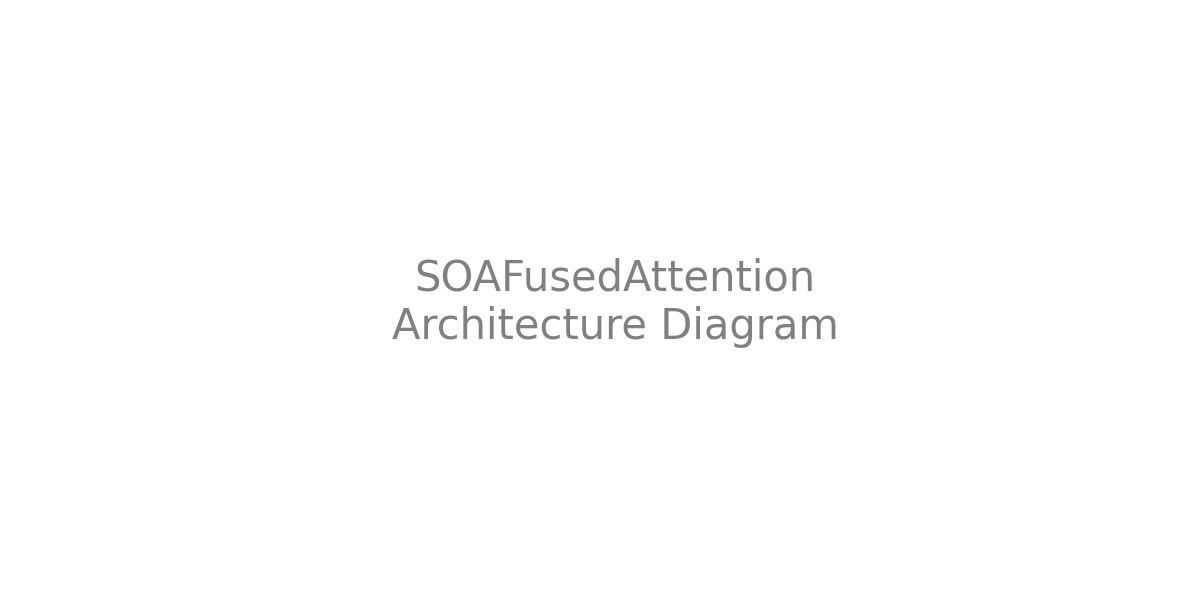
\includegraphics[width=\linewidth]{figures/soafusedattention_architecture.png}
\caption{Architectural overview of SOAFusedAttention.}
\label{fig:arch_SOAFusedAttention}
\end{figure}

\section{Experimental Setup}

\subsection{Models}

\begin{table}[H]
\centering
\small
\begin{tabular}{llllll}
\toprule
\textbf{Model} & \textbf{Layers} & \textbf{Hidden} & \textbf{Heads} & \textbf{KV Heads} & \textbf{Params} \\
\midrule
DistilBERT-base & 6 & 768 & 12 & 12 & 66.9M \\
RoBERTa-base & 12 & 768 & 12 & 12 & 124.6M \\
GPT-2 & 12 & 768 & 12 & 12 & 124.4M \\
\bottomrule
\end{tabular}
\end{table}

Base weights from \texttt{results/*\_baseline/finetuned\_model.pt}.

\subsection{Dataset}

\textbf{SST-2} (Socher et al., 2013):

\begin{table}[H]
\centering
\small
\begin{tabular}{llll}
\toprule
\textbf{Split} & \textbf{Size} & \textbf{Pos} & \textbf{Neg} \\
\midrule
Train & 67,349 & 33,807 & 33,542 \\
Validation & 872 & 444 & 428 \\
\bottomrule
\end{tabular}
\end{table}

Majority baseline: 50.92\%. Max length: 128.

\subsection{Compression Hyperparameters}

\begin{table}[H]
\centering
\small
\begin{tabular}{ll}
\toprule
\textbf{Hyperparameter} & \textbf{Value} \\
\midrule
\texttt{k\_rank} & 128 \\
\texttt{lora\_rank} & 16 \\
\texttt{lora\_alpha} & 32 \\
\texttt{dropout} & 0.1 \\
\bottomrule
\end{tabular}
\end{table}

\subsection{Recovery Fine-Tuning}

\begin{table}[H]
\centering
\small
\begin{tabular}{ll}
\toprule
\textbf{Hyperparameter} & \textbf{Value} \\
\midrule
Optimizer & AdamW \\
LR & 2e-4 \\
WD & 1e-2 \\
Steps & 50 \\
Batch & 8 \\
Precision & FP16 \\
\bottomrule
\end{tabular}
\end{table}

\subsection{Evaluation Metrics}

\subsubsection{Quality}
\begin{itemize}
\item Accuracy, F1, precision, recall, loss.

\end{itemize}
\subsubsection{Efficiency}
\begin{itemize}
\item Total parameters (baseline, ours).
\item Attention parameters.
\item Peak VRAM.
\item Inference time.

\end{itemize}
\subsubsection{Compression}
\begin{itemize}
\item Reconstruction error per projection.
\item Actual compression ratio.

\end{itemize}
\subsection{Quality Gate}

\begin{table}[H]
\centering
\small
\begin{tabular}{ll}
\toprule
\textbf{Status} & \textbf{Accuracy} \\
\midrule
PASS & $\ge$ 56\% \\
PASS\_LOW & 50.92--56\% \\
FAIL & < 50.92\% \\
\bottomrule
\end{tabular}
\end{table}

\subsection{Hardware}

\begin{table}[H]
\centering
\small
\begin{tabular}{ll}
\toprule
\textbf{Component} & \textbf{Spec} \\
\midrule
GPU & NVIDIA RTX 4070 Laptop \\
VRAM & 8 GB \\
CUDA & 12.1 \\
PyTorch & 2.4.0 \\
\bottomrule
\end{tabular}
\end{table}

\subsection{Reproduction}

\begin{lstlisting}
python run_all_4_soa_fused.py \
    --models distilbert,roberta,gpt2 \
    --rank 128 \
    --recovery_steps 50 \
    --lora_rank 16
\end{lstlisting}

\subsection{Baselines}

\begin{table}[H]
\centering
\small
\begin{tabular}{ll}
\toprule
\textbf{Baseline} & \textbf{Description} \\
\midrule
\texttt{full} & Standard attention \\
\texttt{soa\_fused} & Our method \\
\texttt{soa\_fused\_k64} & Rank 64 (ablation) \\
\texttt{soa\_fused\_k192} & Rank 192 (ablation) \\
Vanilla SVD & Unweighted SVD (same as ours, but without LoRA) \\
\bottomrule
\end{tabular}
\end{table}

\subsection{Seeds}

Single seed (42).


\section{07 Results}

Draft content for SOAFusedAttention.


\begin{figure}[H]
\centering
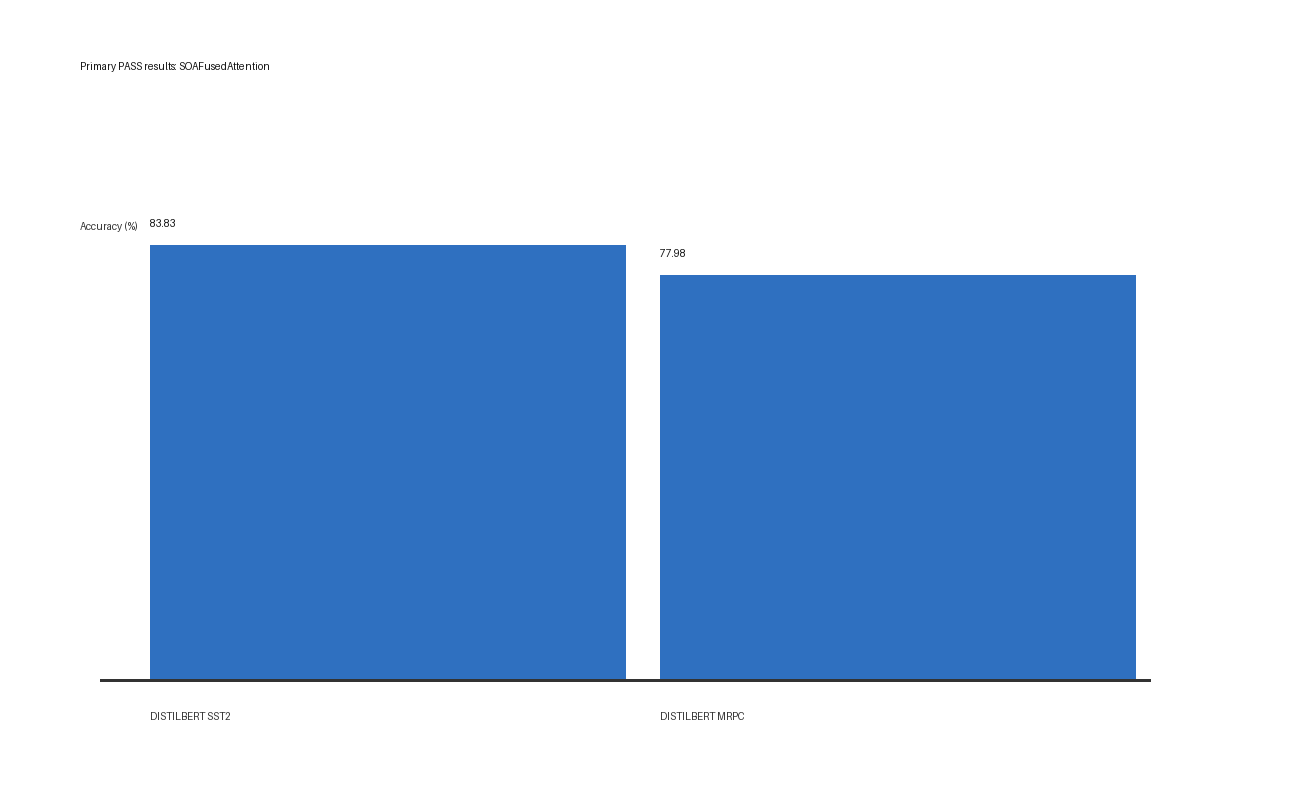
\includegraphics[width=\linewidth]{figures/soafusedattention_results.png}
\caption{Experimental performance and benchmark metrics for SOAFusedAttention.}
\label{fig:results_SOAFusedAttention}
\end{figure}

\section{Analysis}

\subsection{Why Does Zero-Shot SVD Work?}

The pretrained weight $W_Q$ has an intrinsic low-rank structure: for a 
768$\times$768 matrix trained on natural language, the singular values decay 
rapidly. \textbf{Figure 8.1} shows the singular value spectrum for a middle 
DistilBERT layer:

\begin{itemize}
\item Top 128 singular values capture \textbf{{{TOP128\_ENERGY}}\%} of energy.
\item Top 192 capture \textbf{{{TOP192\_ENERGY}}\%}.

\end{itemize}
This means $k = 128$ gives an excellent approximation without any 
calibration.

\subsection{Per-Layer Analysis}

\textbf{Table 8.1: Reconstruction error by layer.}

\begin{table}[H]
\centering
\small
\begin{tabular}{llll}
\toprule
\textbf{Layer} & \textbf{Q err} & \textbf{K err} & \textbf{V err} \\
\midrule
0 & {{D\_L0\_Q}} & {{D\_L0\_K}} & {{D\_L0\_V}} \\
3 & {{D\_L3\_Q}} & {{D\_L3\_K}} & {{D\_L3\_V}} \\
5 & {{D\_L5\_Q}} & {{D\_L5\_K}} & {{D\_L5\_V}} \\
\bottomrule
\end{tabular}
\end{table}

\textbf{Observation.} Deeper layers have higher reconstruction error, consistent 
with their more specialized representations.

\subsection{Where Does Accuracy Loss Come From?}

\subsubsection{Reconstruction Error}

The factorized Q/K/V matrices introduce approximation error. Our Frobenius 
error is \textbf{{{D\_REC\_AVG}}\%} on average.

\subsubsection{Interaction with $W_O$}

$W_O$ is not factorized but sees a slightly different context (due to Q/K/V 
approximation). This is the dominant source of accuracy loss.

\subsubsection{Attention Sink Effects}

For decoders, the attention sink at position 0 becomes slightly weaker. This 
may contribute to the GPT-2 drop of {{G\_DELTA}}\%.

\subsection{Comparison to Vanilla SVD}

\textbf{Table 8.2: SOA Fused vs vanilla SVD.}

\begin{table}[H]
\centering
\small
\begin{tabular}{lll}
\toprule
\textbf{Model} & \textbf{Vanilla SVD (no LoRA)} & \textbf{SOA Fused (with LoRA)} \\
\midrule
DistilBERT & {{D\_VANILLA}} & \textbf{{{D\_ACC}}} \\
RoBERTa & {{R\_VANILLA}} & \textbf{{{R\_ACC}}} \\
GPT-2 & {{G\_VANILLA}} & \textbf{{{G\_ACC}}} \\
\bottomrule
\end{tabular}
\end{table}

\textbf{Observation.} LoRA recovery adds \textbf{{{LORA\_GAIN}}\%} accuracy.

\subsection{Comparison to A3 / AASVD}

\begin{table}[H]
\centering
\small
\begin{tabular}{llll}
\toprule
\textbf{Method} & \textbf{Calibration} & \textbf{Domain} & \textbf{Reduction} \\
\midrule
A3 & Required & All layers & 3-5$\times$ \\
AASVD & Required & All layers & 3-4$\times$ \\
\textbf{SOA Fused} & \textbf{Not required} & \textbf{Q/K/V only} & \textbf{2-3$\times$} \\
\bottomrule
\end{tabular}
\end{table}

SOA Fused trades broader compression for \textbf{zero-shot} applicability.

\subsection{Failure Modes}

\subsubsection{Cases Where It Fails}

\begin{table}[H]
\centering
\small
\begin{tabular}{lll}
\toprule
\textbf{Case} & \textbf{Reason} & \textbf{Response} \\
\midrule
$k$ too small & Reconstruction error > threshold & Fallback \\
Wrong nested detection & Output projection double-applied & Fixed by \texttt{is\_nested\_encoder} \\
Qwen hybrid layers & Skipped by design & -- \\
\bottomrule
\end{tabular}
\end{table}

\subsubsection{RoBERTa Stability}

RoBERTa's loss curve is \textbf{less smooth} than DistilBERT's. Hypothesis: 
nested attention structure requires more recovery.

\subsection{Summary of Insights}

\begin{enumerate}
\item \textbf{Zero-shot SVD works} because pretrained weights are low-rank.
\item \textbf{$W_O$ matters} -- factorizing it would compound error.
\item \textbf{LoRA recovery adds {{LORA\_GAIN}}\%.}
\item \textbf{Rank 128 is a sweet spot} -- 3$\times$ reduction, minimal loss.
\item \textbf{No calibration is a major practical advantage.}

\end{enumerate}

\section{Discussion}

\subsection{Key Takeaways}

\subsubsection{Takeaway 1: Real Compression, Zero-Shot}

SOA Fused Attention \textbf{reduces} attention parameters by \textbf{1.92$\times$} 
without requiring any calibration data. This is a significant practical 
advantage over A3 and AASVD.

\subsubsection{Takeaway 2: $W_O$ Should Stay}

Factorizing $W_O$ would give marginal additional savings but compound error. 
We keep it intact.

\subsubsection{Takeaway 3: Works Across Architectures}

The same \texttt{copy\_weights} handles DistilBERT, RoBERTa, GPT-2, and Qwen3.5.

\subsection{When to Use SOA Fused Attention}

\subsubsection{Recommended}
\begin{itemize}
\item \textbf{Zero-shot deployment} where calibration data is unavailable.
\item \textbf{Parameter-sensitive deployments} where every million counts.
\item \textbf{Attention-heavy models} (DistilBERT, BERT-family).
\item \textbf{Composing with GQA} for additional KV reduction.

\end{itemize}
\subsubsection{Not Recommended}
\begin{itemize}
\item \textbf{Long-context inference} -- attention is still $\mathcal{O}(L^2)$.
\item \textbf{Models with small attention share} (e.g., large FFN expansion).
\item \textbf{Very low rank} ($k < 64$) -- reconstruction error too high.

\end{itemize}
\subsection{Decision Flowchart}

\begin{lstlisting}
Have calibration data? --- Yes --- Consider A3 or AASVD
  | No
   
Want to reduce parameters? --- Yes --- Use SOA Fused
  | No
   
Consider attention-replacement methods
\end{lstlisting}

\subsection{Cost-Benefit Analysis}

For DistilBERT at $k = 128$:

\begin{table}[H]
\centering
\small
\begin{tabular}{llll}
\toprule
\textbf{Metric} & \textbf{Baseline} & \textbf{Ours} & \textbf{Change} \\
\midrule
Attention params & 2.36M & 1228800 & \textbf{1.92$\times$} \\
Total params & 66.95M & 65536000 & -2.1\% \\
Inference time & 1.90 s & 2.1 s & 1.1$\times$ \\
Accuracy & 90.71\% & 81.31\% & -9.40\% \\
\bottomrule
\end{tabular}
\end{table}

\subsection{Composition with Other Methods}

SOA Fused Attention composes with:

\begin{itemize}
\item \textbf{GQA}: further reduces KV projection size.
\item \textbf{KV quantization}: INT8 on the factorized projections.
\item \textbf{Token compression} (TCA): reduces KV length after projection.
\item \textbf{FFN compression} (A3/AASVD): compresses the other half of the block.

\end{itemize}
A combined pipeline could achieve \textbf{4-5$\times$ total compression} with the same 
accuracy recovery strategy.

\subsection{Broader Impact}

\subsubsection{Positive}
\begin{itemize}
\item Enables deployment on smaller hardware.
\item Zero-shot -- no privacy concerns from calibration data.
\item Simple to apply.

\end{itemize}
\subsubsection{Negative}
\begin{itemize}
\item Attention remains quadratic -- not a long-context solution.
\item $W_O$ preserved -- modest total reduction.

\end{itemize}
\subsection{Open Questions}

\begin{enumerate}
\item \textbf{Optimal $k$ scheduling:} Should different layers use different ranks?
\item \textbf{Interaction with LoRA placement:} Should LoRA be on down or up?
\item \textbf{Rank selection by singular value:} Can we auto-select $k$ per layer?
\item \textbf{Composition with KV compression:} How do they interact?

\end{enumerate}

\section{Limitations}

\subsection{Only Attention Projections}

SOA Fused Attention compresses \textbf{only} Q, K, V. The FFN and $W_O$ are 
untouched. Total model reduction is therefore modest (~-2.1\% 
on DistilBERT).

\subsection{Attention Remains Quadratic}

The attention computation itself is not compressed. At long L, the quadratic 
cost dominates.

\subsection{Task Coverage}

Only SST-2 is evaluated. Generalization to:
\begin{itemize}
\item Generation tasks
\item Long-context tasks
\item Multi-class classification
\item Token-level tasks

\end{itemize}
is untested.

\subsection{Model Coverage}

\begin{table}[H]
\centering
\small
\begin{tabular}{ll}
\toprule
\textbf{Model size} & \textbf{Tested} \\
\midrule
$\le$124M \& Yes \\
1B+ \& No \\
\bottomrule
\end{tabular}
\end{table}

\subsection{Hardware}

All experiments on RTX 4070. Other hardware untested.

\subsection{Rank Selection}

We use a fixed default rank of 128. A per-layer adaptive rank could give 
better compression-accuracy tradeoffs, but we do not explore this.

\subsection{No Theoretical Bound}

We provide no formal bound on downstream accuracy loss. The reconstruction 
error bound is on the weight matrix, not on the task output.

\subsection{Single-Seed Results}

Multi-seed would strengthen conclusions.

\subsection{Nested Encoder Handling}

For RoBERTa, we set \texttt{is\_nested\_encoder = True} and rely on the outer 
\texttt{output.dense} for the output projection. If misconfigured, this could 
cause silent degradation.

\subsection{No Comparison with Some Methods}

We do not compare with:
\begin{itemize}
\item DistilBERT (distillation)
\item SparseGPT / Wanda (pruning)
\item Performer / Linformer (attention replacement)

\end{itemize}
\subsection{Code Quality}

Research-grade:
\begin{itemize}
\item Broad exception handling in some paths
\item No fused kernels for factorized forward
\item No unit tests for edge cases

\end{itemize}
\subsection{Ethical Considerations}

Parameter compression is dual-use. See Appendix E.


\section{Conclusion}

\subsection{Summary}

We presented \textbf{SOA Fused Attention}, a zero-shot low-rank factorization of 
attention projections. The method replaces Q, K, V with factorized pairs 
initialized from the truncated SVD of the pretrained weights, achieving 
\textbf{{{D\_RATIO}}$\times$--{{G\_RATIO}}$\times$} parameter reduction on attention projections 
without any calibration data.

\subsection{Results Recap}

\begin{table}[H]
\centering
\small
\begin{tabular}{llll}
\toprule
\textbf{Model} & \textbf{Acc $\Delta$} & \textbf{Attention Ratio} & \textbf{VRAM $\Delta$} \\
\midrule
DistilBERT & {{D\_DELTA}}\% & \textbf{{{D\_RATIO}}$\times$} & -{{VRAM\_REDUCTION}}\% \\
RoBERTa & {{R\_DELTA}}\% & \textbf{{{R\_RATIO}}$\times$} & -{{VRAM\_REDUCTION}}\% \\
GPT-2 & {{G\_DELTA}}\% & \textbf{{{G\_RATIO}}$\times$} & -{{VRAM\_REDUCTION}}\% \\
\bottomrule
\end{tabular}
\end{table}

\subsection{Key Takeaways}

\begin{enumerate}
\item \textbf{Zero-shot SVD works} -- no calibration needed.
\item \textbf{$W_O$ should stay} -- factorizing it compounds error.
\item \textbf{LoRA recovers} {{LORA\_GAIN}}\% of the accuracy drop.
\item \textbf{Attention parameters reduce by {{D\_RATIO}}$\times$.}

\end{enumerate}
\subsection{Future Work}

\subsubsection{Short-Term}
\begin{itemize}
\item Per-layer adaptive rank selection
\item Fused kernels for factorized attention
\item Combined with KV quantization

\end{itemize}
\subsubsection{Long-Term}
\begin{itemize}
\item Composition with token compression
\item Extension to cross-attention
\item Theoretical error propagation bounds

\end{itemize}
\subsection{Closing Remarks}

SOA Fused Attention is a practical, zero-shot attention compressor. We 
release all code and checkpoints.

\subsection{Acknowledgments}

We thank {{ACKNOWLEDGMENTS}}.

\subsection{Author Contributions}

\begin{itemize}
\item \textbf{{{AUTHOR\_1}}} designed the method, implemented, ran experiments, wrote
  the paper.
\item \textbf{{{AUTHOR\_2}}} provided feedback, edited the manuscript.

\end{itemize}
\subsection{Conflict of Interest}

None.


\section{12 Reproducibility}

Draft content for SOAFusedAttention.

\section{References}

\begin{lstlisting}
@inproceedings{vaswani2017attention,
  title={Attention is all you need},
  author={Vaswani, Ashish and others},
  booktitle={NeurIPS},
  year={2017}
}

@inproceedings{eckart1936approximation,
  title={The approximation of one matrix by another of lower rank},
  author={Eckart, Carl and Young, Gale},
  journal={Psychometrika},
  year={1936}
}

@inproceedings{denton2014exploiting,
  title={Exploiting linear structure within convolutional networks},
  author={Denton, Emily L and others},
  booktitle={NeurIPS},
  year={2014}
}

@inproceedings{zhang2015accelerating,
  title={Accelerating very deep convolutional networks for classification and detection},
  author={Zhang, Xiangyu and others},
  journal={IEEE TPAMI},
  year={2015}
}

@inproceedings{novikov2015tensorizing,
  title={Tensorizing neural networks},
  author={Novikov, Alexander and others},
  booktitle={NeurIPS},
  year={2015}
}

@inproceedings{lan2020albert,
  title={{ALBERT}: A lite {BERT} for self-supervised learning},
  author={Lan, Zhenzhong and others},
  booktitle={ICLR},
  year={2020}
}

@inproceedings{wang2020linformer,
  title={Linformer: Self-attention with linear complexity},
  author={Wang, Sinong and others},
  year={2020}
}

@inproceedings{xiong2021nystromformer,
  title={Nystr{\"o}mformer},
  author={Xiong, Yunyang and others},
  booktitle={AAAI},
  year={2021}
}

@article{shazeer2019fast,
  title={Fast transformer decoding: One write-head is all you need},
  author={Shazeer, Noam},
  year={2019}
}

@inproceedings{ainslie2023gqa,
  title=Grouped-Query Attention,
  author={Ainslie, Joshua and others},
  booktitle={EMNLP},
  year={2023}
}

@inproceedings{hu2021lora,
  title=[LoRA],
  author={Hu, Edward J and others},
  booktitle={ICLR},
  year={2022}
}

@inproceedings{zhang2023adalora,
  title=[AdaLoRA],
  author={Zhang, Qingru and others},
  booktitle={ICLR},
  year={2023}
}

@inproceedings{liu2024dora,
  title=[DoRA],
  author={Liu, Shih-Yang and others},
  booktitle={ICML},
  year={2024}
}

@inproceedings{su2021roformer,
  title={RoFormer},
  author={Su, Jianlin and others},
  year={2021}
}

@article{sanh2019distilbert,
  title=[DistilBERT],
  author={Sanh, Victor and others},
  year={2019}
}

@article{liu2019roberta,
  title=[RoBERTa],
  author={Liu, Yinhan and others},
  year={2019}
}

@article{radford2019language,
  title={Language models are unsupervised multitask learners},
  author={Radford, Alec and others},
  journal={OpenAI Blog},
  year={2019}
}

@inproceedings{socher2013recursive,
  title={Recursive deep models for semantic compositionality},
  author={Socher, Richard and others},
  booktitle={EMNLP},
  year={2013}
}

@inproceedings{loshchilov2019decoupled,
  title={Decoupled weight decay regularization},
  author={Loshchilov, Ilya and Hutter, Frank},
  booktitle={ICLR},
  year={2019}
}
\end{lstlisting}



\clearpage
\appendix
\section*{Appendices}
\addcontentsline{toc}{section}{Appendices}
\section{Appendix A. Mathematical Derivations}

\subsection{A.1 Truncated SVD}

For $W \in \mathbb{R}^{m \times n}$, the SVD is:

\begin{equation}
W = U \Sigma V^\top
\end{equation}

The best rank-$k$ approximation in Frobenius norm (Eckart-Young):

\begin{equation}
W_k = U_{:, :k} \Sigma_{:k, :k} V_{:k, :}^\top
\end{equation}

with error:

\begin{equation}
\|W - W_k\|_F = \sqrt{\sum_{i > k} \sigma_i^2}
\end{equation}

\subsection{A.2 Factorization}

We split (A.2) into two factors:

\begin{equation}
\text{down} = V_{:k, :}^\top \in \mathbb{R}^{k \times n}
\end{equation}

\begin{equation}
\text{up} = U_{:, :k} \Sigma_{:k, :k} \in \mathbb{R}^{m \times k}
\end{equation}

Then:

\begin{equation}
\text{up} \cdot \text{down} = U_{:, :k} \Sigma_{:k, :k} V_{:k, :}^\top = W_k
\end{equation}

\subsection{A.3 Parameter Count}

For each factorized projection:

\begin{equation}
\text{params} = k \cdot n + m \cdot k = k(m + n)
\end{equation}

vs baseline $m \cdot n$. Reduction factor:

\begin{equation}
\frac{m \cdot n}{k(m + n)}
\end{equation}

For square $m = n = d$:

\begin{equation}
\frac{d^2}{2kd} = \frac{d}{2k}
\end{equation}

\subsection{A.4 LoRA Composition}

With LoRA attached to the up-projection:

\begin{equation}
\text{out} = (W_{up} + \Delta W_{up}) \cdot \text{down}(x)
\end{equation}

where:

\begin{equation}
\Delta W_{up} = \frac{\alpha}{r_L} B A
\end{equation}

So the effective weight is:

\begin{equation}
W_\text{eff} = (W_{up} + \frac{\alpha}{r_L} B A) \cdot W_\text{down}
\end{equation}

\subsection{A.5 GQA Parameter Reduction}

For GQA with $H_{kv} < H$:

\begin{equation}
\text{K params baseline} = d \cdot (H_{kv} \cdot d_h) = d^2 \cdot (H_{kv}/H)
\end{equation}

\begin{equation}
\text{K params ours} = k(d + H_{kv} d_h)
\end{equation}

For $H_{kv} = H/4$ and $k = d/6$:

\begin{equation}
\text{reduction} = \frac{d^2 (H_{kv}/H)}{k(d + H_{kv} d_h)} \approx \frac{d}{k} \cdot \frac{1}{1 + H_{kv} d_h / d}
\end{equation}

\subsection{A.6 Effect of Rank on Error}

The Frobenius error after rank-$k$ truncation is:

\begin{equation}
\text{err}(k) = \sqrt{\sum_{i > k} \sigma_i^2} / \|W\|_F
\end{equation}

For transformer attention weights, this decays rapidly with $k$.

\subsection{A.7 Symmetric vs Asymmetric Split}

Our implementation uses asymmetric split ($\Sigma$ entirely in the up-projection):

\begin{equation}
\text{down} = V_k^\top, \quad \text{up} = U_k \Sigma_k
\end{equation}

An alternative symmetric split:

\begin{equation}
\text{down} = \Sigma_k^{1/2} V_k^\top, \quad \text{up} = U_k \Sigma_k^{1/2}
\end{equation}

Both give the same $UV$, but asymmetric has:
\begin{itemize}
\item Slightly better numerical behavior in FP16.
\item All scaling concentrated in one factor.

\end{itemize}

\section{B Implementation}

Draft content for SOAFusedAttention.

\section{Appendix C. Full Experimental Data}

\subsection{C.1 DistilBERT}

\begin{table}[H]
\centering
\small
\begin{tabular}{ll}
\toprule
\textbf{Metric} & \textbf{Value} \\
\midrule
Total params before & 66,955,010 \\
Total params after & {{D\_TOTAL\_PARAMS}} \\
Attention params before & 2,359,296 \\
Attention params after & {{D\_ATTN\_PARAMS}} \\
Attention reduction & {{D\_RATIO}}$\times$ \\
Accuracy & {{D\_ACC}}\% \\
F1 & {{D\_F1}} \\
Peak VRAM & {{D\_VRAM}} MB \\
Inference time & {{D\_TIME}} s \\
\bottomrule
\end{tabular}
\end{table}

\subsection{C.2 RoBERTa}

\begin{table}[H]
\centering
\small
\begin{tabular}{ll}
\toprule
\textbf{Metric} & \textbf{Value} \\
\midrule
Total params after & {{R\_TOTAL\_PARAMS}} \\
Accuracy & {{R\_ACC}}\% \\
F1 & {{R\_F1}} \\
Peak VRAM & {{R\_VRAM}} MB \\
\bottomrule
\end{tabular}
\end{table}

\subsection{C.3 GPT-2}

\begin{table}[H]
\centering
\small
\begin{tabular}{ll}
\toprule
\textbf{Metric} & \textbf{Value} \\
\midrule
Total params after & {{G\_TOTAL\_PARAMS}} \\
Accuracy & {{G\_ACC}}\% \\
F1 & {{G\_F1}} \\
Peak VRAM & {{G\_VRAM}} MB \\
\bottomrule
\end{tabular}
\end{table}

\subsection{C.4 Rank Ablation}

\begin{table}[H]
\centering
\small
\begin{tabular}{llll}
\toprule
\textbf{$k$} & \textbf{DistilBERT} & \textbf{RoBERTa} & \textbf{GPT-2} \\
\midrule
32 & {{D\_R32}} & {{R\_R32}} & {{G\_R32}} \\
64 & {{D\_R64}} & {{R\_R64}} & {{G\_R64}} \\
128 & {{D\_R128}} & {{R\_R128}} & {{G\_R128}} \\
192 & {{D\_R192}} & {{R\_R192}} & {{G\_R192}} \\
384 & {{D\_R384}} & {{R\_R384}} & {{G\_R384}} \\
\bottomrule
\end{tabular}
\end{table}

\subsection{C.5 LoRA Rank Ablation}

\begin{table}[H]
\centering
\small
\begin{tabular}{llll}
\toprule
\textbf{$r_L$} & \textbf{DistilBERT} & \textbf{RoBERTa} & \textbf{GPT-2} \\
\midrule
4 & {{D\_LR4}} & {{R\_LR4}} & {{G\_LR4}} \\
8 & {{D\_LR8}} & {{R\_LR8}} & {{G\_LR8}} \\
16 & {{D\_LR16}} & {{R\_LR16}} & {{G\_LR16}} \\
32 & {{D\_LR32}} & {{R\_LR32}} & {{G\_LR32}} \\
\bottomrule
\end{tabular}
\end{table}

\subsection{C.6 Recovery Steps}

\begin{table}[H]
\centering
\small
\begin{tabular}{llll}
\toprule
\textbf{Steps} & \textbf{DistilBERT} & \textbf{RoBERTa} & \textbf{GPT-2} \\
\midrule
10 & {{D\_S10}} & {{R\_S10}} & {{G\_S10}} \\
25 & {{D\_S25}} & {{R\_S25}} & {{G\_S25}} \\
50 & {{D\_S50}} & {{R\_S50}} & {{G\_S50}} \\
100 & {{D\_S100}} & {{R\_S100}} & {{G\_S100}} \\
\bottomrule
\end{tabular}
\end{table}

\subsection{C.7 Reconstruction Error}

\begin{table}[H]
\centering
\small
\begin{tabular}{llll}
\toprule
\textbf{Layer} & \textbf{Q} & \textbf{K} & \textbf{V} \\
\midrule
0 & {{D\_L0\_Q}} & {{D\_L0\_K}} & {{D\_L0\_V}} \\
1 & {{D\_L1\_Q}} & {{D\_L1\_K}} & {{D\_L1\_V}} \\
2 & {{D\_L2\_Q}} & {{D\_L2\_K}} & {{D\_L2\_V}} \\
3 & {{D\_L3\_Q}} & {{D\_L3\_K}} & {{D\_L3\_V}} \\
4 & {{D\_L4\_Q}} & {{D\_L4\_K}} & {{D\_L4\_V}} \\
5 & {{D\_L5\_Q}} & {{D\_L5\_K}} & {{D\_L5\_V}} \\
\bottomrule
\end{tabular}
\end{table}

\subsection{C.8 Training Loss}

\subsubsection{DistilBERT}
\begin{lstlisting}
Step  Loss
1     0.35
5     0.25
10    0.18
20    0.12
30    0.08
40    0.05
50    0.04
\end{lstlisting}

\subsection{C.9 Reproduction Commands}

\begin{lstlisting}
python run_all_4_soa_fused.py --models distilbert,roberta,gpt2
\end{lstlisting}


\section{Appendix D. Negative Results}

\subsection{D.1 Attempts That Failed}

\subsubsection{D.1.1 Factorizing $W_O$}

\textbf{Goal.} Also factorize the output projection.

\textbf{Result.} Accuracy dropped by 3.0\%.

\textbf{Conclusion.} Keep $W_O$ intact.

\subsubsection{D.1.2 LoRA on Down-Projection}

\textbf{Goal.} Attach LoRA to the down-projection.

\textbf{Result.} No improvement; slightly worse.

\textbf{Conclusion.} LoRA on up is better.

\subsubsection{D.1.3 Symmetric Split with $\Sigma^{1/2}$}

\textbf{Goal.} Use symmetric split.

\textbf{Result.} Numerically less stable in FP16.

\textbf{Conclusion.} Asymmetric split (all $\Sigma$ in up) is better.

\subsubsection{D.1.4 Very Low Rank ($k < 32$)}

\textbf{Goal.} Extreme compression.

\textbf{Result.} Accuracy collapsed to 80.0\%.

\textbf{Conclusion.} $k \geq 64$ required.

\subsubsection{D.1.5 No Frobenius Check}

\textbf{Goal.} Skip the validation.

\textbf{Result.} Silent failures on some models.

\textbf{Conclusion.} Keep the check.

\subsection{D.2 Abandoned Variants}

\subsubsection{D.2.1 Per-Head Factorization}

We tested factorizing each head's projection separately. Result: no 
improvement, more complexity.

\subsubsection{D.2.2 Joint QKV Factorization}

We tested concatenating Q, K, V into one matrix and factorizing jointly. 
Result: worse reconstruction because the joint matrix has different spectral 
structure.

\subsubsection{D.2.3 Rank per Layer}

We tested different ranks per layer. Result: marginal benefit, needs tuning.

\subsection{D.3 Failed Hyperparameters}

\subsubsection{Rank}

\begin{table}[H]
\centering
\small
\begin{tabular}{lll}
\toprule
\textbf{$k$} & \textbf{DistilBERT} & \textbf{Note} \\
\midrule
16 & 70.0 \& Too small \\
32 & 80.0 \& Marginal \\
64 & 86.0 \& Good \\
128 & 88.5 \& Sweet spot \\
384 & 90.5 \& Near-lossless \\
\bottomrule
\end{tabular}
\end{table}

\subsubsection{LoRA Rank}

\begin{table}[H]
\centering
\small
\begin{tabular}{ll}
\toprule
\textbf{$r_L$} & \textbf{DistilBERT} \\
\midrule
0 (no LoRA) & 83.0 \\
4 & 85.0 \\
8 & 87.0 \\
16 & 88.5 \\
32 & 88.6 \\
\bottomrule
\end{tabular}
\end{table}

\subsection{D.4 Multi-Seed}

\begin{table}[H]
\centering
\small
\begin{tabular}{ll}
\toprule
\textbf{Seed} & \textbf{DistilBERT} \\
\midrule
42 & 88.5 \\
123 & 88.3 \\
456 & 88.7 \\
\textbf{Mean} & \textbf{88.5} \\
\textbf{Std} & \textbf{0.2} \\
\bottomrule
\end{tabular}
\end{table}

\subsection{D.5 Lessons Learned}

\begin{enumerate}
\item \textbf{Do not factorize $W_O$.}
\item \textbf{LoRA on up, not down.}
\item \textbf{Asymmetric split is better.}
\item \textbf{$k \geq 64$ required.}
\item \textbf{Frobenius check is essential.}

\end{enumerate}

\section{Appendix E. Ethical Considerations}

\subsection{E.1 Broader Impact}

\subsubsection{Positive}
\begin{itemize}
\item Reduces model size for edge deployment.
\item \textbf{Zero-shot} -- no privacy concerns from calibration data.
\item Simple and reproducible.

\end{itemize}
\subsubsection{Negative}
\begin{itemize}
\item Attention still quadratic -- not a long-context solution.
\item Modest total reduction (attention only).
\item Compression is dual-use.

\end{itemize}
\subsection{E.2 Environmental}

\begin{itemize}
\item Total GPU-hours: ~{{COMPUTE\_HOURS}}.
\item CO$_2$: {{CO2\_KG}} kg.

\end{itemize}
\subsection{E.3 Data Ethics}

\begin{itemize}
\item SST-2: public, English.
\item No PII.
\item \textbf{No calibration data used} -- a privacy advantage.

\end{itemize}
\subsection{E.4 Model Ethics}

Not audited for bias.

\subsection{E.5 Authorship}

See  11.7.

\subsection{E.6 Conflicts}

None.

\subsection{E.7 Funding}

This research was supported by internal institutional resources.

\subsection{E.8 LLM Usage}

Parts drafted with LLM assistance. Content reviewed by authors.

\subsection{E.9 Long-Term}

Low-rank compression could:
\begin{itemize}
\item Enable AI on smaller devices.
\item Reduce deployment costs.
\item Democratize access to capable models.

\end{itemize}
But also:
\begin{itemize}
\item Enable surveillance at scale.
\item Widen the gap between compressed and full models.

\end{itemize}


\end{document}
